\competentie
{% competentieformulier
	\competentieformulier
	{% toelichting
		You have acquired knowledge and skills which are vital to your becoming an ICT professional. You are able to assess the knowledge you have gained for its relevance. You use this knowledge to make well-informed decisions on how to carry out assignments and solve the issues you may encounter in professional practice. In so doing, you work methodically, set criteria which must be met by the result, and work in accordance with professional (international) ICT standards. You have an enterprising attitude.
	}
	{% deelcompetenties
		methodical approach,% 
		ability to apply (scientific) knowledge and insights,% 
		providing a high-quality product/service,% 
		showing an enterprising attitude.% 
	}
	{%
		Proof
	}
	{%
		This competency will always be assessed, both in your final project and in your final project report.
	}
	{% verwijzing naar bewijs
		Figure~\ref{fig:terraform},
		Figure~\ref{fig:react},
		Figure~\ref{fig:kubernets}
	}
}
{% bewijzen
	\bewijs
	{% naam
		% TODO 
		Learning new skills to assist my current employer better.
	}
	{% starr
		\starr
		{% betreft
			showing an enterprising attitude.% 
		}
		{% datum
			25-06-2022
		}
		{% situatie

			When the client for the inventory system came to me to create the application I had a choice which langauge to choose and which framework.

			I'm have more experience with for example with a normal old school deployment of applications.
			But to improve and assist my current employer more I decided to learn new skills that are actively used at VanMoof.
		}
		{% taak
			Look which software and skills are used at VanMoof and use this assignment to learn and apply those skills.
		}
		{% activiteiten
			At VanMoof we currently use a lot of kubernetes, terraform and other cloud related stuff.
			Also as a data engineer I have to create a lot of ETL's.

			There are a lot of integrations and I looked for the most used and decided to improve upon those skills.
		}
		{% resultaat
			I came to the understanding that the most essential skills that I'm currently lacking are kubernetes and terraform.

			I took and finished a cursuses about kubernetes, terraform and react and decided to use them in the application.

			The result was an application build with those previouse mentioned technologies.
			except for terraform, I will reflect on why in the next section.
		}
		{% reflectie
			I should have done better research on the usage of the technologies.
			Kubernetes and react fit well with the application context.

			But terraform didn't, after learning and finishing the cursus I came to a better understanding of terraform.
			It's not a tool to manage network infrastructures but a tool to manages cloud infrastructures.
			This means that it is able to create cloud instances such as databases or secrets for a big organization.
			It translates the code to actual products and creates them.
			For a single application there is no need to use terraform.

			I'm now however able to support VanMoof with terraform by using the knowledge learned for the cursus.
		}

		{
		}
	}
	{% bewij
		\begin{figure}
			\begin{center}
				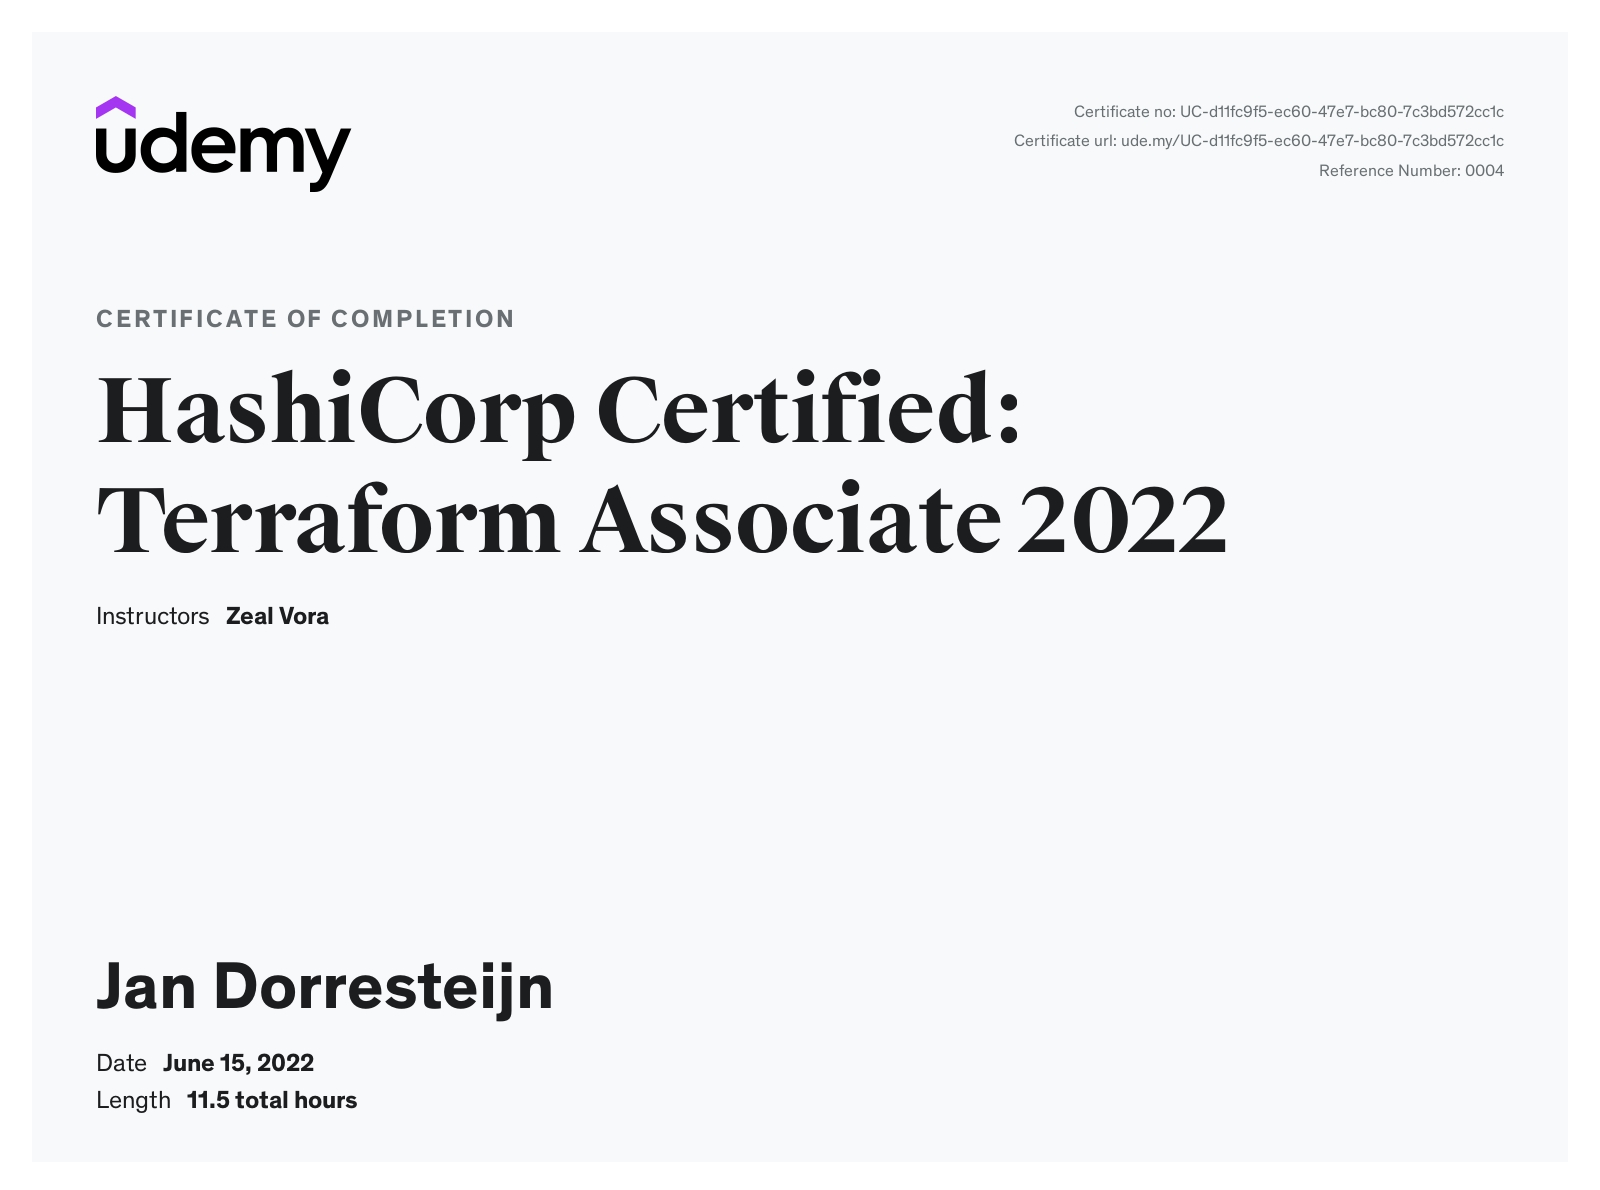
\includegraphics[width=0.95\textwidth]{images/terra.jpg}
			\end{center}
			\caption{Terraform}
			\label{fig:terraform}
		\end{figure}
		\begin{figure}
			\begin{center}
				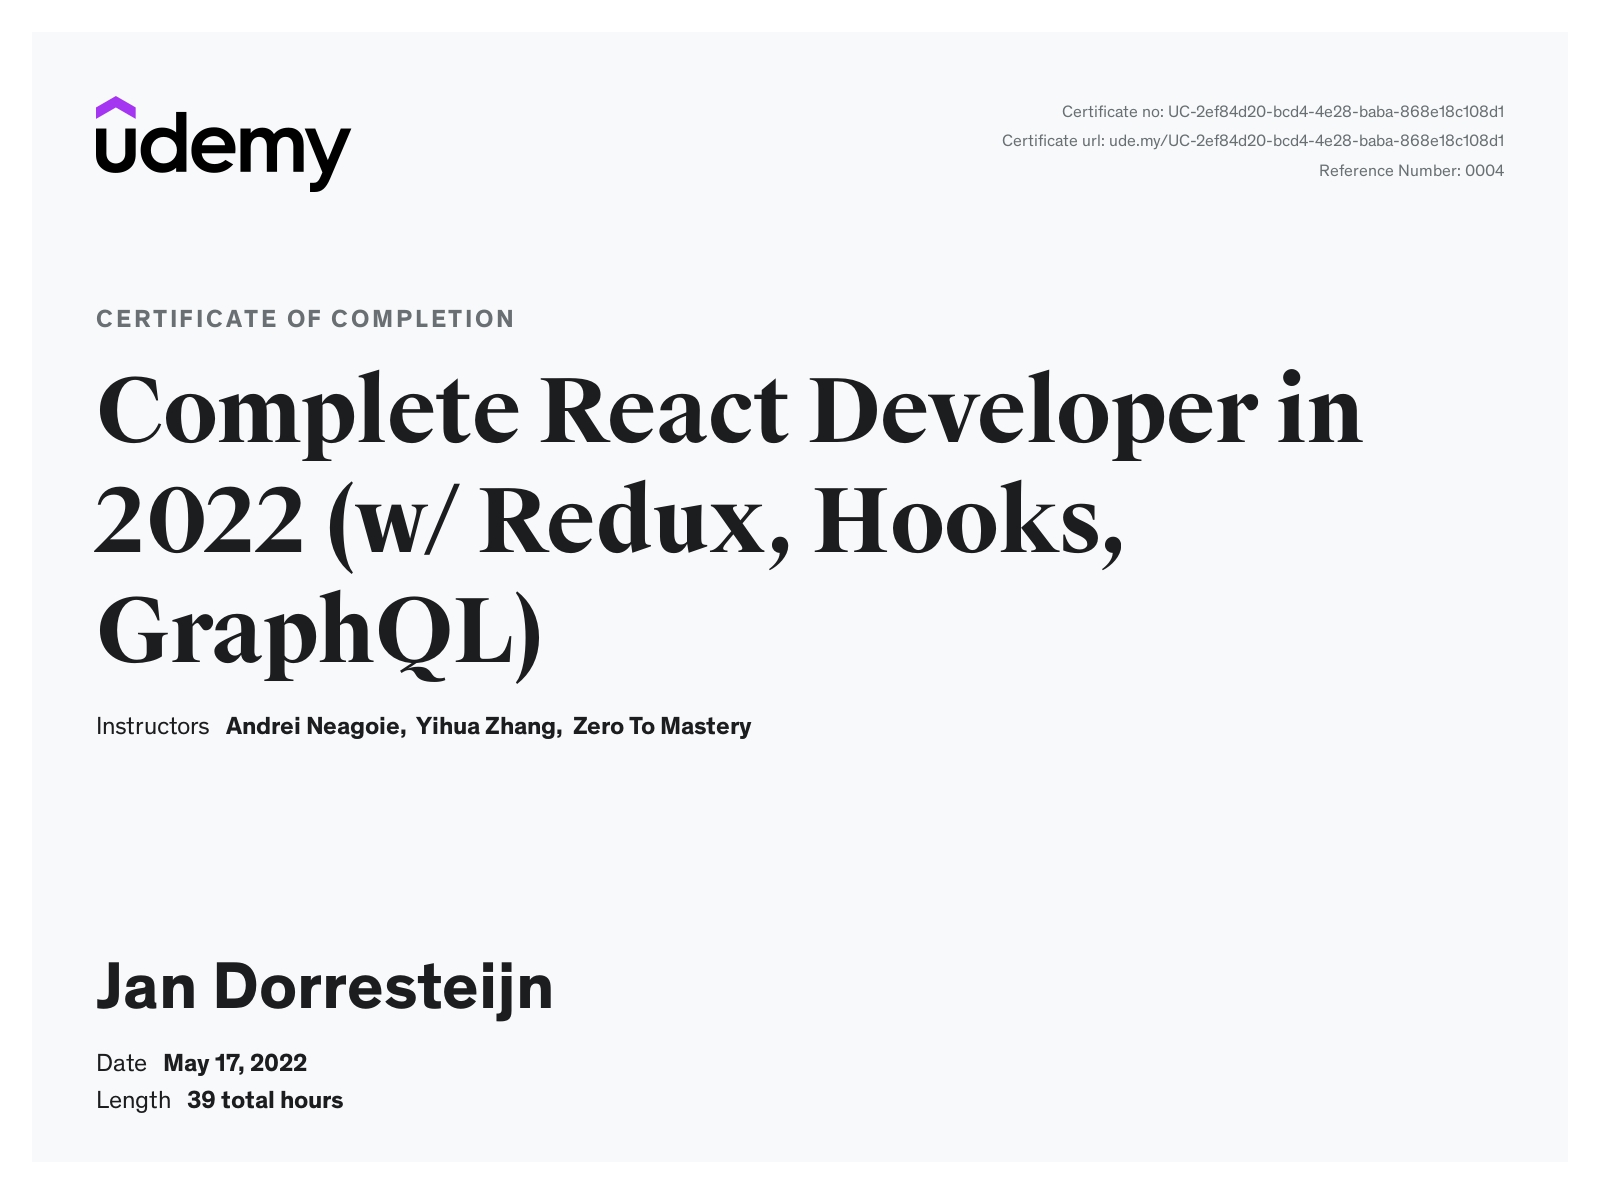
\includegraphics[width=0.95\textwidth]{images/react.jpg}
			\end{center}
			\caption{React}
			\label{fig:react}
		\end{figure}
		\begin{figure}
			\begin{center}
				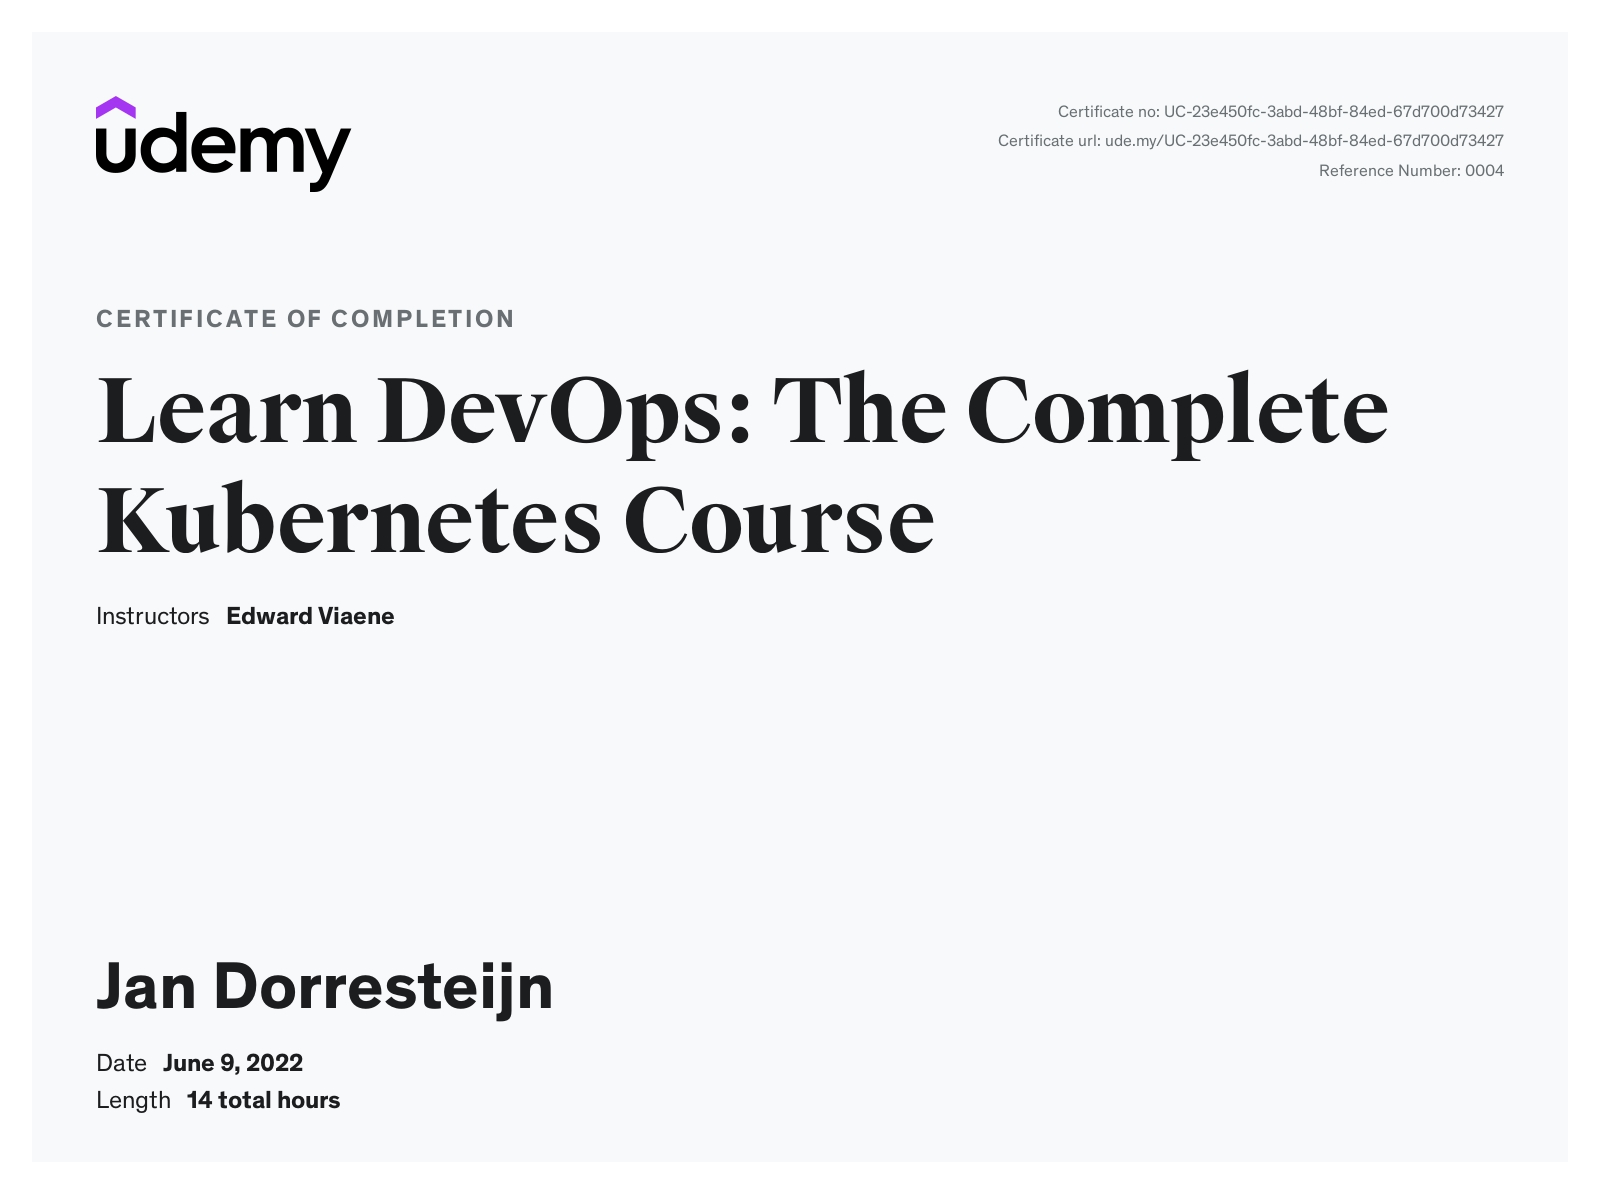
\includegraphics[width=0.95\textwidth]{images/kube.jpg}
			\end{center}
			\caption{Kubernetes}
			\label{fig:kubernets}
		\end{figure}

	},
}

